% Provenance (never printed): cycle 4 SVT, "La planete Terre": the history of
% the Earth read in the rocks, relative dating (superposition, recoupement,
% inclusion, continuite paleontologique), the ages of the Earth, eras and
% periods, the scale of geological time; see sources/book1/PROVENANCE.md.
% Book 1, grade 7, chapter 5.
% Vocabulary guard: owns relative dating / absolute age, the four principles,
% unconformity, era and geological period, the geological time scale. The
% method of radiometric dating is the physics books' and grade 12's: told
% here in two sentences, never defined. Fossils as evidence of evolution are
% the biology books' (one sentence of prose). "Ice age" is grade 8's: not used.
\chapter{As idades da Terra}\label{ch:g7:geological-time}

Em junho~de~1788, o geólogo escocês James Hutton e dois amigos, o
matemático John Playfair e o químico James Hall, visitaram Siccar Point,
uma ponta rochosa ``lavada até a \omterm{def:g3:stones-pebbles-sand:rock}{rocha} nua pelo \omterm{def:g2:water-on-earth:ocean}{mar}'' no \omterm{def:g1:landscapes-around-us:water}{litoral} da
Escócia. Na parte de baixo da \omterm{def:g3:stones-pebbles-sand:rock}{rocha}, eles viram camadas cinzentas em pé,
quase verticais. Por cima delas havia camadas de arenito vermelho,
levemente inclinadas. Hutton explicou o que tinha acontecido: as camadas
cinzentas tinham sido depositadas na horizontal no fundo de um \omterm{def:g2:water-on-earth:ocean}{mar},
depois empurradas até ficarem em pé, depois desgastadas, antes de a \omterm{def:g3:stones-pebbles-sand:sand}{areia}
vermelha ser depositada por cima delas. Cada uma dessas etapas precisou
de um tempo imenso. Playfair escreveu mais tarde: ``A mente parecia ficar
tonta de olhar tão longe no abismo do tempo.''
% ledger: ncse:siccar-point

\begin{omfigure}
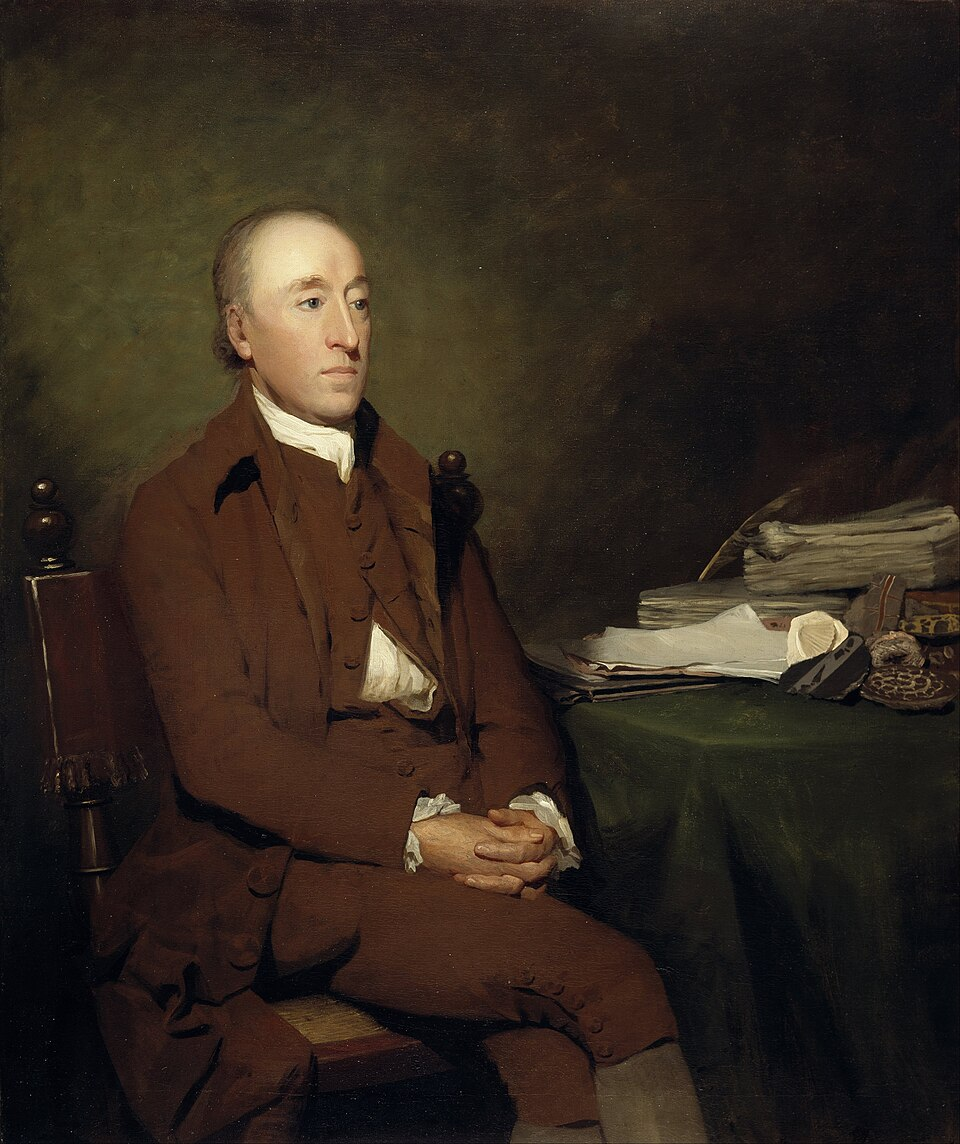
\includegraphics[width=0.3\linewidth]{images/book1/g7-hutton.jpg}

{\small James Hutton (1726--1797), pintado por Henry Raeburn. Hutton
via cada camada como um intervalo de tempo, com a mais antiga embaixo,
onde quer que as camadas não tenham sido viradas. Retrato em domínio público, via Wikimedia
Commons.}
% ledger: commons:hutton-portrait, usgs:hutton-smith
\label{fig:g7:geological-time:hutton}
\end{omfigure}

Como saber que \omterm{def:g3:stones-pebbles-sand:rock}{rocha} é mais velha que outra, sem nenhuma data escrita
nela? Qual é a idade da Terra? E como imaginar uma história tão longa?

\begin{recall}
Os \omterm{def:g7:sediments-and-fossils:sediment}{sedimentos} se depositam em camadas, uma em cima da outra, e endurecem
em \omterm{def:g6:rocks-and-minerals:rock-families}{rocha sedimentar}; os \omterm{def:g7:sediments-and-fossils:fossil}{fósseis} são os restos ou os vestígios de seres
vivos conservados na \omterm{def:g3:stones-pebbles-sand:rock}{rocha} (\cref{ch:g7:sediments-and-fossils}). Uma
\emph{\omterm{def:g7:earthquakes:fault}{falha}} é uma ruptura nas \omterm{def:g3:stones-pebbles-sand:rock}{rochas} ao longo da qual os dois lados se
deslocaram (\cref{ch:g7:earthquakes}). O granito é uma \emph{\omterm{def:g6:rocks-and-minerals:rock-families}{rocha
ígnea}}: ele se forma quando a \omterm{def:g3:stones-pebbles-sand:rock}{rocha} derretida esfria devagar, bem fundo
embaixo da terra; o xisto é uma \emph{\omterm{def:g6:rocks-and-minerals:rock-families}{rocha metamórfica}}, transformada
pelo calor e pela pressão; um conglomerado é uma \omterm{def:g6:rocks-and-minerals:rock-families}{rocha sedimentar} feita
de \omterm{def:g3:stones-pebbles-sand:pebble}{seixos} cimentados uns nos outros (\cref{ch:g6:rocks-and-minerals}).
\end{recall}

\section{O que veio primeiro?}

Os historiadores conseguem pôr acontecimentos em ordem mesmo sem as suas
datas. A Primeira Guerra Mundial veio antes da Segunda: os nomes delas
dizem isso. A televisão ainda não estava nas casas quando os irmãos
Wright voaram pela primeira vez, em 1903, mas muita gente assistiu aos
primeiros passos na Lua pela televisão em 1969: então o voo veio
primeiro, depois a televisão nas casas, e depois a Lua. Juntar pistas e
compará-las basta para encontrar a ordem. Para quase toda a história da
Terra não existe nenhum registro escrito, e os geólogos trabalham do
mesmo jeito: eles usam as pistas guardadas nas \omterm{def:g3:stones-pebbles-sand:rock}{rochas}.
% ledger: usgs:events-order

\begin{definition}[Datação relativa e idade absoluta]\label{def:g7:geological-time:relative-dating}
A \emph{datação relativa}\index{datacao relativa@datação relativa} põe as \omterm{def:g3:stones-pebbles-sand:rock}{rochas} e os
acontecimentos em ordem, do mais velho ao mais novo, sem dizer há quantos
anos eles aconteceram: esta \omterm{def:g3:stones-pebbles-sand:rock}{rocha} é mais velha que aquela. Uma
\emph{idade absoluta}\index{idade absoluta} é uma idade dada em número de
anos, por exemplo ``\num{300} milhões de anos''.
\end{definition}

\section{Quatro princípios para pôr as rochas em ordem}

Quatro princípios simples fazem a maior parte do trabalho da \omterm{def:g7:geological-time:relative-dating}{datação
relativa}. Eles estão ilustrados abaixo, em quatro penhascos imaginários. O primeiro foi enunciado por Nicolau Steno em 1669; Hutton se apoiou nele no fim do século~XVIII.
% ledger: usgs:hutton-smith, og:stratigraphy-principles

\begin{omfigure}
\tikzset{
  trilo/.pic={\fill[black!65] (0,0) ellipse (0.13 and 0.085);
              \draw[white, line width=0.3pt] (-0.11,0.028) -- (0.11,0.028) (-0.11,-0.028) -- (0.11,-0.028);},
  ammo/.pic={\draw[black!75, line width=0.45pt] (0,0) circle (0.1) (0,0) circle (0.062) (0,0) circle (0.028);}
}
\begin{minipage}[t]{0.49\linewidth}\centering
\begin{tikzpicture}[font=\footnotesize]
  \fill[lith sandstone] (0,0) rectangle (4.4,0.6);
  \fill[lith shale] (0,0.6) rectangle (4.4,1.2);
  \fill[lith limestone] (0,1.2) rectangle (4.4,1.8);
  \fill[lith sandstone] (0,1.8) rectangle (4.4,2.4);
  \foreach \k in {1,2,3,4} \node[fill=white, inner sep=1pt] at (0.35,0.6*\k-0.3) {\k};
  \draw (0,0) rectangle (4.4,2.4);
  \foreach \y in {0.6,1.2,1.8} \draw[contact] (0,\y) -- (4.4,\y);
  \draw[-{Stealth}, line width=0.8pt] (4.75,0.1) -- (4.75,2.3);
  \node[anchor=west] at (4.85,2.2) {mais nova};
  \node[anchor=west] at (4.85,0.2) {mais velha};
\end{tikzpicture}

{\small (a) Superposição: a camada 1 se formou primeiro, a camada 4 por último.}
\end{minipage}\hfill
\begin{minipage}[t]{0.49\linewidth}\centering
\begin{tikzpicture}[font=\footnotesize]
  % left block, below the fault
  \begin{scope}
    \clip (0,0) -- (3.75,0) -- (3.25,2.4) -- (0,2.4) -- cycle;
    \fill[lith sandstone] (0,0) rectangle (5,0.6);
    \fill[lith shale] (0,0.6) rectangle (5,1.2);
    \fill[lith limestone] (0,1.2) rectangle (5,1.8);
    \fill[lith granite] (1.2,0) -- (1.85,0) -- (1.75,0.9) -- (1.9,1.8) -- (1.15,1.8) -- (1.3,0.9) -- cycle;
    \fill[lith sandstone] (0,1.8) rectangle (5,2.4);
    \foreach \y in {0.6,1.2} {\draw[contact] (0,\y) -- (1.25,\y); \draw[contact] (1.8,\y) -- (5,\y);}
    \draw[contact] (1.2,0) -- (1.3,0.9) -- (1.15,1.8) (1.85,0) -- (1.75,0.9) -- (1.9,1.8);
    \draw[contact] (0,1.8) -- (5,1.8);
  \end{scope}
  % right block, moved down along the fault
  \begin{scope}
    \clip (3.75,0) -- (5,0) -- (5,2.05) -- (3.32,2.05) -- cycle;
    \fill[lith sandstone] (3,-0.35) rectangle (5,0.25);
    \fill[lith shale] (3,0.25) rectangle (5,0.85);
    \fill[lith limestone] (3,0.85) rectangle (5,1.45);
    \fill[lith sandstone] (3,1.45) rectangle (5,2.05);
    \foreach \y in {0.25,0.85,1.45} \draw[contact] (3,\y) -- (5,\y);
  \end{scope}
  \draw (0,0) -- (5,0) -- (5,2.05) -- (3.32,2.05) (3.25,2.4) -- (0,2.4) -- (0,0);
  \draw[fault] (3.75,0) -- (3.25,2.4);
  \node[anchor=south, fill=white, inner sep=1pt] at (1.5,2.45) {granito};
  \draw[black!70] (1.5,2.45) -- (1.52,1.6);
  \node[anchor=south] at (4.2,2.45) {falha};
  \draw[black!70] (4.0,2.45) -- (3.4,1.75);
\end{tikzpicture}

{\small (b) Relações de corte: o granito é mais novo que as três camadas
que ele corta, e mais velho que a camada de cima; a \omterm{def:g7:earthquakes:fault}{falha}, que quebra
todas elas, é a mais nova.}
\end{minipage}

\bigskip
\begin{minipage}[t]{0.49\linewidth}\centering
\begin{tikzpicture}[font=\footnotesize]
  \fill[lith granite] (0,0) -- (4.4,0) -- (4.4,1.05) .. controls (3.4,0.95) and (2.6,1.2) .. (1.6,1.0) .. controls (0.9,0.88) and (0.4,1.1) .. (0,1.0) -- cycle;
  \fill[lith conglomerate] (0,2.4) -- (4.4,2.4) -- (4.4,1.05) .. controls (3.4,0.95) and (2.6,1.2) .. (1.6,1.0) .. controls (0.9,0.88) and (0.4,1.1) .. (0,1.0) -- cycle;
  \foreach \x/\y/\a/\b in {0.5/1.35/0.2/0.12, 1.3/1.25/0.16/0.1, 2.1/1.45/0.22/0.13, 2.9/1.3/0.17/0.11, 3.7/1.4/0.2/0.12, 0.9/1.8/0.15/0.1, 2.5/1.95/0.17/0.1, 3.4/1.85/0.14/0.09}
    \filldraw[fill=omLithGranite, draw=black!70, line width=0.3pt] (\x,\y) ellipse [x radius=\a, y radius=\b];
  \draw[unconformity] (0,1.0) .. controls (0.4,1.1) and (0.9,0.88) .. (1.6,1.0) .. controls (2.6,1.2) and (3.4,0.95) .. (4.4,1.05);
  \draw (0,0) rectangle (4.4,2.4);
  \node[fill=white, inner sep=1pt] at (2.2,0.45) {granito};
  \node[anchor=west] at (4.5,1.7) {conglomerado};
  \node[anchor=west, align=left] at (4.5,1.15) {seixos de\\granito};
  \draw[black!70] (4.5,1.15) -- (3.85,1.4);
\end{tikzpicture}

{\small (c) Inclusão: os \omterm{def:g3:stones-pebbles-sand:pebble}{seixos} de granito são mais velhos que o
conglomerado que os contém.}
\end{minipage}\hfill
\begin{minipage}[t]{0.49\linewidth}\centering
\begin{tikzpicture}[font=\footnotesize]
  % place A
  \fill[lith shale] (0,0) rectangle (1.3,0.8);
  \fill[lith limestone] (0,0.8) rectangle (1.3,1.6);
  \fill[lith sandstone] (0,1.6) rectangle (1.3,2.4);
  \draw (0,0) rectangle (1.3,2.4); \draw[contact] (0,0.8) -- (1.3,0.8) (0,1.6) -- (1.3,1.6);
  \foreach \x in {0.3,0.65,1.0} {\pic at (\x,0.4) {trilo}; \pic at (\x,1.2) {ammo};}
  \node[anchor=south] at (0.65,2.45) {lugar A};
  % place B
  \fill[lith sandstone] (3.6,0.4) rectangle (4.9,1.0);
  \fill[lith shale] (3.6,1.0) rectangle (4.9,2.0);
  \fill[lith limestone] (3.6,0) rectangle (4.9,0.4);
  \draw (3.6,0) rectangle (4.9,2.0); \draw[contact] (3.6,0.4) -- (4.9,0.4) (3.6,1.0) -- (4.9,1.0);
  \foreach \x in {3.9,4.25,4.6} {\pic at (\x,0.7) {trilo}; \pic at (\x,1.5) {ammo};}
  \node[anchor=south] at (4.25,2.45) {lugar B};
  \draw[dashed, black!70] (1.3,0.8) -- (3.6,1.0) (1.3,0) -- (3.6,0.4) (1.3,1.6) -- (3.6,2.0);
  \pic at (2.15,-0.3) {trilo}; \node[anchor=west] at (2.3,-0.3) {trilobita};
  \pic at (2.15,2.3) {ammo}; \node[anchor=west] at (2.3,2.3) {amonite};
\end{tikzpicture}

{\small (d) Sucessão dos \omterm{def:g7:sediments-and-fossils:fossil}{fósseis}: as camadas com os mesmos \omterm{def:g7:sediments-and-fossils:fossil}{fósseis} têm a
mesma idade, embora as suas \omterm{def:g3:stones-pebbles-sand:rock}{rochas} sejam diferentes.}
\end{minipage}

\medskip
{\small Os quatro princípios da \omterm{def:g7:geological-time:relative-dating}{datação relativa}, em quatro penhascos
imaginários.}
% ledger: usgs:hutton-smith, usgs:cross-cutting, nps:cross-cutting, eli:relative-dating, usgs:fossil-succession
\label{fig:g7:geological-time:principles}
\end{omfigure}

\begin{definition}[Princípio da superposição]\label{def:g7:geological-time:superposition}
O \emph{princípio da superposição}\index{superposicao, principio da@superposição, princípio da}:
numa pilha de \omterm{def:g7:sediments-and-fossils:layer}{camadas sedimentares} que não foi virada, cada camada é mais
nova que a camada de baixo e mais velha que a camada de cima. A camada
mais velha fica embaixo, a mais nova em cima.
\end{definition}
% ledger: usgs:hutton-smith, eli:relative-dating

\begin{definition}[Princípio das relações de corte]\label{def:g7:geological-time:cross-cutting}
O \emph{princípio das relações de corte}\index{relacoes de corte, principio das@relações de corte, princípio das}: uma \omterm{def:g3:stones-pebbles-sand:rock}{rocha} ou uma estrutura que corta
outras \omterm{def:g3:stones-pebbles-sand:rock}{rochas} é mais nova que as \omterm{def:g3:stones-pebbles-sand:rock}{rochas} que ela corta. Uma massa de
granito que atravessa camadas, uma \omterm{def:g7:earthquakes:fault}{falha} que as quebra e uma superfície
de \omterm{def:g5:water-shapes-the-land:erosion}{erosão} que as desgasta são todas mais novas que essas camadas.
\end{definition}
% ledger: usgs:cross-cutting, nps:cross-cutting, eli:relative-dating

\begin{definition}[Princípio da inclusão]\label{def:g7:geological-time:inclusion}
O \emph{princípio da inclusão}\index{inclusao, principio da@inclusão, princípio da}: os pedaços
de uma \omterm{def:g3:stones-pebbles-sand:rock}{rocha} encontrados dentro de outra \omterm{def:g3:stones-pebbles-sand:rock}{rocha} são mais velhos que a
\omterm{def:g3:stones-pebbles-sand:rock}{rocha} que os contém. Os \omterm{def:g3:stones-pebbles-sand:pebble}{seixos} de um conglomerado já existiam antes de o
conglomerado se formar em volta deles.
\end{definition}
% ledger: eli:relative-dating

\begin{definition}[Princípio da sucessão dos fósseis]\label{def:g7:geological-time:fossil-succession}
O \emph{princípio da sucessão dos fósseis}\index{sucessao dos fosseis, principio da@sucessão dos fósseis, princípio da}: os tipos de animais e de plantas encontrados como \omterm{def:g7:sediments-and-fossils:fossil}{fósseis} mudam
das camadas mais velhas para as mais novas, sempre na mesma ordem. As
\omterm{def:g3:stones-pebbles-sand:rock}{rochas} que guardam os mesmos tipos de \omterm{def:g7:sediments-and-fossils:fossil}{fósseis} têm a mesma idade, mesmo
quando estão longe umas das outras.
\end{definition}
% ledger: usgs:fossil-succession


O \omterm{def:g7:geological-time:superposition}{princípio da superposição} só vale para camadas que não foram viradas:
em alguns lugares, a formação das \omterm{def:g1:landscapes-around-us:landform}{montanhas} dobrou uma pilha de camadas
com tanta força que ela ficou de cabeça para baixo. Os geólogos então
procuram pistas que mostrem em que sentido as camadas se formaram --- as
pegadas e as marcas de ondulação, por exemplo, ficam na superfície de cima
de uma camada. O \omterm{def:g7:geological-time:fossil-succession}{princípio da sucessão dos fósseis} funciona porque a vida
na Terra mudou ao longo do tempo: a maioria dos \omterm{def:g7:sediments-and-fossils:fossil}{fósseis} pertence a
espécies que não vivem mais em lugar nenhum. Por que a vida mudou é
contado nos livros de biologia.
% ledger: eli:relative-dating, usgs:fossil-succession, nps:ripple-marks

\begin{history}[William Smith, o construtor de canais]
Entre 1785 e 1800, enquanto Hutton trabalhava na Escócia, William Smith,
um engenheiro inglês que construía canais, colecionava as conchas \omterm{def:g7:sediments-and-fossils:fossil}{fósseis}
dos calcários e dos folhelhos que ele escavava. Ele descobriu que cada
camada guardava os seus próprios \omterm{def:g7:sediments-and-fossils:fossil}{fósseis}, diferentes dos das camadas de
cima e de baixo. Usando esses \omterm{def:g7:sediments-and-fossils:fossil}{fósseis} como marcadores, ele conseguia
reconhecer a mesma camada onde quer que ela aparecesse, e desenhou alguns
dos primeiros \omterm{def:g2:drawing-to-map:map}{mapas} geológicos de grandes regiões.
\end{history}
% ledger: usgs:hutton-smith

\section{Lacunas no registro}

Em Siccar Point, as camadas cinzentas e o arenito vermelho não se
formaram um logo depois do outro. Entre os dois, as camadas cinzentas
foram inclinadas e levantadas, e depois desgastadas durante muito tempo,
e nenhuma camada dessa época ficou guardada. A superfície entre os dois
conjuntos de \omterm{def:g3:stones-pebbles-sand:rock}{rochas} é uma lacuna no registro.

\begin{definition}[Discordância]\label{def:g7:geological-time:unconformity}
Uma \emph{discordância}\index{discordancia@discordância} é uma superfície de \omterm{def:g5:water-shapes-the-land:erosion}{erosão}
entre dois conjuntos de \omterm{def:g3:stones-pebbles-sand:rock}{rochas} formados em épocas muito diferentes: as
\omterm{def:g3:stones-pebbles-sand:rock}{rochas} mais velhas foram desgastadas antes de as mais novas serem
depositadas por cima delas. Ela marca um longo período do qual nenhuma
camada ficou guardada.
\end{definition}
% ledger: ncse:siccar-point, eli:relative-dating

\begin{omfigure}
\begin{tikzpicture}[font=\footnotesize, x=1cm, y=1cm]
  \def\stripes#1#2#3{% x0, width, top: vertical layers
    \foreach \i in {0,...,7} {
      \pgfmathsetmacro{\xa}{#1+\i*#2/8}
      \pgfmathsetmacro{\xb}{#1+(\i+1)*#2/8}
      \ifodd\i\def\lithc{omLithSchist}\else\def\lithc{omLithShale}\fi
      \fill[\lithc] (\xa,0) rectangle (\xb,#3);
      \draw[black!55, line width=0.3pt] (\xa,0) -- (\xa,#3);
    }}
  % 1: flat layers under the sea
  \fill[omSea!70] (0,1.6) rectangle (3.4,2.4);
  \foreach \k in {0,...,3} {
    \ifodd\k\def\lithc{omLithSchist}\else\def\lithc{omLithShale}\fi
    \fill[\lithc] (0,0.4*\k) rectangle (3.4,0.4*\k+0.4);
    \draw[black!55, line width=0.3pt] (0,0.4*\k) -- (3.4,0.4*\k);
  }
  \draw (0,0) rectangle (3.4,2.4);
  \node[anchor=north, align=center] at (1.7,-0.1) {1. Camadas depositadas\\na horizontal num mar};
  % 2: pushed up on end
  \begin{scope}[xshift=3.9cm]
    \begin{scope}
      \clip (0,0) -- (3.4,0) -- (3.4,1.7) -- (2.6,2.2) -- (1.6,1.75) -- (0.9,2.3) -- (0,1.8) -- cycle;
      \stripes{0}{3.4}{2.4}
    \end{scope}
    \draw (0,1.8) -- (0.9,2.3) -- (1.6,1.75) -- (2.6,2.2) -- (3.4,1.7);
    \draw (0,1.8) -- (0,0) -- (3.4,0) -- (3.4,1.7);
    \node[anchor=north, align=center] at (1.7,-0.1) {2. Empurradas até ficarem\\em pé, acima do mar};
  \end{scope}
  % 3: worn flat
  \begin{scope}[xshift=7.8cm]
    \stripes{0}{3.4}{1.3}
    \draw[unconformity] (0,1.3) -- (3.4,1.3);
    \draw (0,1.3) -- (0,0) -- (3.4,0) -- (3.4,1.3);
    \node[anchor=north, align=center] at (1.7,-0.1) {3. Desgastadas\\durante muito tempo};
  \end{scope}
  % 4: new layers on top
  \begin{scope}[xshift=11.7cm]
    \stripes{0}{3.4}{1.3}
    \fill[om lith={red!22}{om sand}] (0,1.3) rectangle (3.4,1.85);
    \fill[om lith={red!30}{om sand}] (0,1.85) rectangle (3.4,2.4);
    \draw[contact] (0,1.85) -- (3.4,1.85);
    \draw[unconformity, line width=0.9pt] (0,1.3) -- (3.4,1.3);
    \draw (0,0) rectangle (3.4,2.4);
    \node[anchor=north, align=center] at (1.7,-0.1) {4. Novas camadas por cima:\\uma discordância};
  \end{scope}
  \foreach \x in {3.45,7.35,11.25} \draw[-{Stealth}, line width=0.7pt] (\x,1.2) -- (\x+0.4,1.2);
\end{tikzpicture}

{\small Como se forma uma \omterm{def:g7:geological-time:unconformity}{discordância} como a de Siccar Point. A linha
ondulada é a \omterm{def:g7:geological-time:unconformity}{discordância}: o longo tempo das etapas 2 e 3 não deixou
nenhuma camada.}
% ledger: ncse:siccar-point
\label{fig:g7:geological-time:unconformity}
\end{omfigure}

\section{Ler a história de uma região}

Um corte geológico mostra as \omterm{def:g3:stones-pebbles-sand:rock}{rochas} como elas apareceriam num corte feito
bem para baixo, no chão. Os quatro princípios o transformam numa história.

\begin{method}[Pôr em ordem os acontecimentos de um corte geológico]\label{met:g7:geological-time:ordering}
\begin{enumerate}
  \item Encontre as \omterm{def:g3:stones-pebbles-sand:rock}{rochas} mais velhas: as que são cortadas por todo o
        resto, ou que ficam embaixo da pilha.
  \item Encontre cada \omterm{def:g3:stones-pebbles-sand:rock}{rocha} ou estrutura que corta outras (um granito,
        uma \omterm{def:g7:earthquakes:fault}{falha}, uma superfície de \omterm{def:g5:water-shapes-the-land:erosion}{erosão}): ela é mais nova que tudo o
        que ela corta.
  \item Leia as camadas de baixo para cima (superposição), e procure as
        \omterm{def:g7:geological-time:unconformity}{discordâncias}, onde falta tempo.
  \item As camadas são depositadas na horizontal: se estão inclinadas ou
        dobradas, o dobramento veio depois delas.
  \item Escreva os acontecimentos em ordem, do mais velho ao mais novo,
        com a pista de cada um.
\end{enumerate}
\end{method}
% ledger: eli:relative-dating, usgs:cross-cutting, nps:cross-cutting

\begin{omfigure}
\begin{tikzpicture}
\begin{axis}[x=1.4cm, y=0.007cm, xmin=0, xmax=10, ymin=-500, ymax=300,
  axis on top, tick label style={font=\scriptsize}, label style={font=\small},
  xlabel={distância para leste a partir de E (km)}, ylabel={altitude (m)},
  ytick={-400,-200,0,200}, clip mode=individual]
\addplot[lith schist, draw=black, line width=0.3pt, even odd rule] table {figdata/out/grade-7-varden_history-unit-schist.dat};
\addplot[lith granite, draw=black, line width=0.3pt, even odd rule] table {figdata/out/grade-7-varden_history-unit-granite.dat};
\addplot[om lith={icsTriassic!35}{om sand}, draw=black, line width=0.3pt, even odd rule] table {figdata/out/grade-7-varden_history-unit-sandstone.dat};
\addplot[om lith={icsJurassic!40}{om limestone}, draw=black, line width=0.3pt, even odd rule] table {figdata/out/grade-7-varden_history-unit-limestone.dat};
\addplot[om lith={icsJurassic!15}{om shale}, draw=black, line width=0.3pt, even odd rule] table {figdata/out/grade-7-varden_history-unit-shale.dat};
\addplot[om lith={icsCretaceous!35}{om limestone}, draw=black, line width=0.3pt, even odd rule] table {figdata/out/grade-7-varden_history-unit-chalk.dat};
\addplot[lith alluvium, draw=black, line width=0.3pt, even odd rule] table {figdata/out/grade-7-varden_history-unit-alluvium.dat};
\addplot[omThm, line width=1.3pt] table {figdata/out/grade-7-varden_history-base.dat};
\addplot[black, line width=0.8pt] table {figdata/out/grade-7-varden_history-ground.dat};
\addplot[fault, line width=1.3pt] table {figdata/out/grade-7-varden_history-fault.dat};
\node[font=\small, above right] at (axis cs:0,300) {E (oeste)};
\node[font=\small, above left] at (axis cs:10,300) {F (leste)};
\end{axis}
\end{tikzpicture}

\smallskip
{\small\setlength{\tabcolsep}{4pt}
\begin{tabular}{@{}llll@{}}
\tikz\fill[lith schist, draw=black] (0,0) rectangle (0.5,0.3); xisto &
\tikz\fill[lith granite, draw=black] (0,0) rectangle (0.5,0.3); granito &
\tikz\fill[om lith={icsTriassic!35}{om sand}, draw=black] (0,0) rectangle (0.5,0.3); arenito &
\tikz\fill[om lith={icsJurassic!40}{om limestone}, draw=black] (0,0) rectangle (0.5,0.3); calcário \\
\tikz\fill[om lith={icsJurassic!15}{om shale}, draw=black] (0,0) rectangle (0.5,0.3); folhelho &
\tikz\fill[om lith={icsCretaceous!35}{om limestone}, draw=black] (0,0) rectangle (0.5,0.3); giz &
\tikz\fill[lith alluvium, draw=black] (0,0) rectangle (0.5,0.3); \omterm{def:g3:stones-pebbles-sand:sand}{areia} de \omterm{def:g1:landscapes-around-us:water}{rio} &
\tikz\draw[omThm, line width=1.3pt] (0,0.15) -- (0.5,0.15); base do arenito \\
\end{tabular}}

\smallskip
{\small O corte E--F, de oeste (E) para leste (F), atravessando o meio
das Colinas de Varden, a região inventada desta coleção, passando pelo
seu granito. A linha preta grossa é a \omterm{def:g7:earthquakes:fault}{falha}. As \omterm{def:g4:world-physical-map:altitude}{altitudes} estão esticadas
5 vezes em relação às distâncias, para que as camadas fiquem mais fáceis
de ver.}
% ledger: (invented region: figdata/shared/region.py, section E--F by figdata/grade-7/varden_history.py)
\label{fig:g7:geological-time:section}
\end{omfigure}

\begin{example}[A história das Colinas de Varden]\label{ex:g7:geological-time:varden}
Aplique o método ao corte E--F.
\begin{enumerate}
  \item O xisto é cortado pelo granito e fica embaixo de todas as
        camadas: é a \omterm{def:g3:stones-pebbles-sand:rock}{rocha} mais velha.
  \item O granito corta o xisto (relações de corte), então ele é mais
        novo. Ele não corta nenhuma das camadas de cima: é mais velho que
        o arenito.
  \item O granito esfriou bem fundo embaixo da terra, e mesmo assim a
        base do arenito, que fica sobre o xisto, chega ao topo do granito:
        as \omterm{def:g3:stones-pebbles-sand:rock}{rochas} que os cobriam foram desgastadas antes de a \omterm{def:g3:stones-pebbles-sand:sand}{areia}
        chegar. A base do arenito é uma \omterm{def:g7:geological-time:unconformity}{discordância}.
  \item O arenito, o calcário, o folhelho e o giz foram depositados nessa
        ordem (superposição).
  \item As camadas foram depositadas na horizontal, mas agora estão
        dobradas, arqueadas por cima do granito e curvadas para baixo
        mais a leste: o dobramento veio depois do giz.
  \item A \omterm{def:g7:earthquakes:fault}{falha} quebra todas as camadas dobradas: ela é mais nova que o
        dobramento.
  \item A superfície do chão de hoje corta tudo, e a \omterm{def:g3:stones-pebbles-sand:sand}{areia} de \omterm{def:g1:landscapes-around-us:water}{rio} fica
        por cima dela: a \omterm{def:g5:water-shapes-the-land:erosion}{erosão} e os \omterm{def:g1:landscapes-around-us:water}{rios} são os acontecimentos mais
        recentes.
\end{enumerate}
A história, do mais velho ao mais novo: o xisto; o granito; a \omterm{def:g5:water-shapes-the-land:erosion}{erosão}; as
quatro camadas; o dobramento; a \omterm{def:g7:earthquakes:fault}{falha}; a \omterm{def:g5:water-shapes-the-land:erosion}{erosão} de hoje e a \omterm{def:g3:stones-pebbles-sand:sand}{areia} de \omterm{def:g1:landscapes-around-us:water}{rio}.
% ledger: (invented region: figdata/grade-7/varden_history.py main table)
\end{example}

A \omterm{def:g7:geological-time:relative-dating}{datação relativa} dá a ordem dos acontecimentos, mas não as suas datas,
nem quanto durou cada um: o método diz que a \omterm{def:g7:earthquakes:fault}{falha} é mais nova que o giz,
e não por quantos anos.

\section{Eras e períodos}

A sucessão dos \omterm{def:g7:sediments-and-fossils:fossil}{fósseis} permite aos geólogos fazer corresponder camadas do
mundo inteiro. Juntando as suas observações, eles dividiram a história da
Terra em intervalos de tempo, do mesmo jeito que os historiadores falam
de séculos e de reinados.
% ledger: usgs:hutton-smith, usgs:fossil-succession

\begin{omfigure}
\begin{tikzpicture}[font=\footnotesize]
\begin{axis}[name=long, x dir=reverse, xmin=0, xmax=4600, ymin=0, ymax=1,
  width=14.3cm, height=1.7cm, scale only axis, axis y line=none, axis x line*=bottom,
  xtick={4500,4000,3000,2000,1000}, tick label style={font=\scriptsize}, clip=false]
  \pgfplotsinvokeforeach{Hadean,Archean,Proterozoic,Phanerozoic}{
    \addplot[fill=ics#1, draw=black!70, line width=0.3pt] table {figdata/out/grade-7-time_scale-bar-#1.dat};}
  \addplot[draw=none, nodes near coords, point meta=explicit symbolic,
    every node near coord/.style={anchor=center, font=\scriptsize, fill=white, fill opacity=0.85, text opacity=1, inner sep=1pt}]
    table[row sep=\\, x=age, y=y, meta=name] {age y name\\ 4299 0.5 Hadeano\\ 3265.5 0.5 Arqueano\\ 1519.4 0.5 Proterozoico\\ 269.4 0.5 Fanerozoico\\ };
  \coordinate (z1) at (axis cs:538.8,0);
  \coordinate (z2) at (axis cs:0,0);
\end{axis}
\begin{axis}[at={(long.south west)}, anchor=north west, yshift=-1.3cm,
  x dir=reverse, xmin=0, xmax=540, ymin=0, ymax=3.2,
  width=14.3cm, height=3.6cm, scale only axis, axis y line=none, axis x line*=bottom,
  xtick={500,400,300,200,100,0}, tick label style={font=\scriptsize},
  xlabel={milhões de anos atrás}, label style={font=\small}, clip=false]
  \pgfplotsinvokeforeach{Paleozoic,Mesozoic,Cenozoic}{
    \addplot[fill=ics#1, draw=black!70, line width=0.3pt] table[x=age, y expr=2.4+0.8*\thisrow{y}] {figdata/out/grade-7-time_scale-bar-#1.dat};}
  \pgfplotsinvokeforeach{Cambrian,Ordovician,Silurian,Devonian,Carboniferous,Permian,Triassic,Jurassic,Cretaceous,Paleogene,Neogene,Quaternary}{
    \addplot[fill=ics#1, draw=black!70, line width=0.3pt] table[x=age, y expr=2.4*\thisrow{y}] {figdata/out/grade-7-time_scale-bar-#1.dat};}
  \addplot[draw=none, nodes near coords, point meta=explicit symbolic,
    every node near coord/.style={anchor=center, font=\footnotesize\bfseries, fill=white, fill opacity=0.85, text opacity=1, inner sep=1pt}]
    table[row sep=\\, x=age, y expr=2.8, meta=name] {age y name\\ 395.351 0.5 Paleozoico\\ 158.951 0.5 Mesozoico\\ 33 0.5 Cenozoico\\ };
  \addplot[draw=none, nodes near coords, point meta=explicit symbolic, x filter/.expression={x<2 ? nan : x},
    every node near coord/.style={anchor=center, rotate=90, font=\scriptsize, fill=white, fill opacity=0.85, text opacity=1, inner sep=1pt}]
    table[row sep=\\, x=age, y expr=1.2, meta=name] {age y name\\ 512.825 0.5 Cambriano\\ 464.975 0.5 Ordoviciano\\ 431.36 0.5 Siluriano\\ 389.24 0.5 Devoniano\\ 328.88 0.5 Carbonífero\\ 275.401 0.5 Permiano\\ 226.651 0.5 Triássico\\ 172.25 0.5 Jurássico\\ 104.55 0.5 Cretáceo\\ 44.52 0.5 Paleógeno\\ 12.81 0.5 Neógeno\\ 1.29 0.5 Quaternário\\ };
  \addplot[draw=none, nodes near coords, point meta=explicit symbolic, x filter/.expression={x<2 ? x : nan},
    every node near coord/.style={anchor=west, xshift=3pt, font=\scriptsize}]
    table[row sep=\\, x=age, y expr=1.2, meta=name] {age y name\\ 512.825 0.5 Cambriano\\ 464.975 0.5 Ordoviciano\\ 431.36 0.5 Siluriano\\ 389.24 0.5 Devoniano\\ 328.88 0.5 Carbonífero\\ 275.401 0.5 Permiano\\ 226.651 0.5 Triássico\\ 172.25 0.5 Jurássico\\ 104.55 0.5 Cretáceo\\ 44.52 0.5 Paleógeno\\ 12.81 0.5 Neógeno\\ 1.29 0.5 Quaternário\\ };
  \coordinate (w1) at (axis cs:540,3.2);
  \coordinate (w2) at (axis cs:0,3.2);
\end{axis}
\draw[dashed, black!60] (z1) -- ++(0,-0.5) -- (w1) (z2) -- (w2);
\end{tikzpicture}

{\small A \omterm{def:g7:geological-time:time-scale}{escala do tempo geológico}, nas cores da tabela internacional.
Em cima: a história inteira da Terra. Embaixo: a sua última parte, o
Fanerozoico, esticada: as suas três \omterm{def:g7:geological-time:era-period}{eras} e os doze \omterm{def:g7:geological-time:era-period}{períodos geológicos}.
Idades em milhões de anos antes de hoje.}
% ledger: ics:base.Hadean, ics:base.Archean, ics:base.Proterozoic, ics:base.Paleozoic, ics:base.Mesozoic, ics:base.Cenozoic, ics:colour.Hadean (figdata/grade-7/time_scale.py reads every ics base and colour row of the shared ledger)
\label{fig:g7:geological-time:scale}
\end{omfigure}

\begin{definition}[Era e período geológico]\label{def:g7:geological-time:era-period}
Uma \emph{era}\index{era} é um longo intervalo da história da Terra,
definido pelo tipo geral de vida que existia nessa época: o Paleozoico, o
Mesozoico e o Cenozoico. Cada era é dividida em intervalos mais curtos,
os \emph{períodos geológicos}\index{periodo geologico@período geológico}, como o
Jurássico ou o Cretáceo.
\end{definition}
% ledger: usgs:hutton-smith

\begin{definition}[Escala do tempo geológico]\label{def:g7:geological-time:time-scale}
A \emph{escala do tempo geológico}\index{escala do tempo geologico@escala do tempo geológico} é a lista
das divisões da história da Terra em ordem --- os longos intervalos do
seu começo, as \omterm{def:g7:geological-time:era-period}{eras} e os \omterm{def:g7:geological-time:era-period}{períodos geológicos} ---, com a idade, em anos,
do começo de cada uma. Uma tabela internacional dá a cada divisão o seu
nome, a sua idade e a sua cor.
\end{definition}
% ledger: ics:base.Hadean, ics:colour.Hadean


As três \omterm{def:g7:geological-time:era-period}{eras} são recentes em comparação com a história inteira. O
Paleozoico começou há \num{538.8} milhões de anos, quando os \omterm{def:g7:sediments-and-fossils:fossil}{fósseis} de
animais com concha ficaram comuns; o Mesozoico durou de \num{251.9} a
\num{66} milhões de anos atrás; o Cenozoico, a \omterm{def:g7:geological-time:era-period}{era} em que vivemos,
começou há \num{66} milhões de anos. Antes do Paleozoico se estendem três
longos intervalos, o Hadeano, o Arqueano e o Proterozoico: eles cobrem
cerca de 88~\% da história da Terra, mas os seus \omterm{def:g7:sediments-and-fossils:fossil}{fósseis} são raros. Os dinossauros viveram no Mesozoico: eles dominaram
durante mais de \num{100} milhões de anos, e, no fim do Cretáceo, todos
eles tinham desaparecido.
% ledger: ics:base.Paleozoic, ics:base.Mesozoic, ics:base.Cenozoic, usgs:numeric-scale, usgs:dinosaurs-extinct (figdata/grade-7/time_scale.py main table: 88.1 %)

As Colinas de Varden cabem nessa escala. O seu arenito é do Triássico, o
seu calcário e o seu folhelho são do Jurássico, o seu giz é do Cretáceo:
os três pertencem ao Mesozoico. No corte E--F, eles estão desenhados em
versões claras das cores da tabela.
% ledger: (invented region: figdata/shared/region.py UNITS)

\section{A história da Terra num ano}

Números em bilhões de anos são difíceis de imaginar. Imagine, em vez
disso, a história inteira da Terra espremida num único ano. A Terra se
forma em 1º~de~janeiro, à meia-noite; hoje é a última badalada da
meia-noite no fim de 31~de~dezembro. A Terra tem cerca de \num{4540}
milhões de anos, então um dia desse ano vale $4540 \div 365$, cerca de
\num{12.4} milhões de anos.
% ledger: usgs:age-earth (figdata/grade-7/earth_calendar.py)

\begin{omfigure}
\begin{tikzpicture}[font=\footnotesize]
\begin{axis}[xmin=0, xmax=365, ymin=0, ymax=1, width=15.2cm, height=0.9cm,
  scale only axis, axis y line=none, axis x line=none, clip=false]
  \addplot[ycomb, black!60, line width=0.4pt] table[x=day, y expr=1] {figdata/out/grade-7-earth_calendar-days.dat};
  \draw[black!70] (axis cs:0,0) rectangle (axis cs:365,1);
  \addplot[draw=none, nodes near coords, point meta=explicit symbolic,
    every node near coord/.style={anchor=center, font=\scriptsize}]
    table[row sep=\\, x=mid, y expr=0.5, meta=name] {mid name\\ 15.5 jan\\ 45 fev\\ 74.5 mar\\ 105 abr\\ 135.5 mai\\ 166 jun\\ 196.5 jul\\ 227.5 ago\\ 258 set\\ 288.5 out\\ 319 nov\\ 349.5 dez\\ };
  \addplot[only marks, mark=triangle*, mark size=2.6pt, omThm, mark options={rotate=180}]
    table[x=day, y expr=1.18] {figdata/out/grade-7-earth_calendar.dat};
  \addplot[draw=none, nodes near coords, point meta=explicit symbolic, x filter/.expression={x>200 ? nan : x},
    every node near coord/.style={anchor=west, rotate=40, xshift=2pt, yshift=4pt, font=\scriptsize}]
    table[row sep=\\, x=day, y expr=1.18, meta=tag] {day tag\\ 0 {1º de janeiro: a Terra se forma}\\ 41 {11 de fevereiro: as rochas mais velhas}\\ 83.61 {25 de março: os fósseis mais velhos}\\ 321.68 {18 de novembro: conchas comuns}\\ 359.69 {26 de dezembro: fim dos dinossauros}\\ };
  \addplot[draw=none, nodes near coords, point meta=explicit symbolic, x filter/.expression={x>200 ? x : nan},
    every node near coord/.style={anchor=east, rotate=-40, xshift=-2pt, yshift=4pt, font=\scriptsize}]
    table[row sep=\\, x=day, y expr=1.18, meta=tag] {day tag\\ 0 {1º de janeiro: a Terra se forma}\\ 41 {11 de fevereiro: as rochas mais velhas}\\ 83.61 {25 de março: os fósseis mais velhos}\\ 321.68 {18 de novembro: conchas comuns}\\ 359.69 {26 de dezembro: fim dos dinossauros}\\ };
\end{axis}
\end{tikzpicture}

{\small A história da Terra como um ano do calendário: cada mês vale cerca
de \num{373} milhões de anos, cada dia cerca de \num{12.4} milhões de
anos. As datas são calculadas a partir das idades dos acontecimentos.}
% ledger: usgs:age-earth, usgs:oldest-rocks, usgs:numeric-scale, ics:base.Paleozoic, ics:base.Paleogene (figdata/grade-7/earth_calendar.py)
\label{fig:g7:geological-time:calendar}
\end{omfigure}

As \omterm{def:g3:stones-pebbles-sand:rock}{rochas} mais velhas encontradas até hoje chegam em 11~de~fevereiro; os
\omterm{def:g7:sediments-and-fossils:fossil}{fósseis} mais velhos conhecidos, em 25~de~março. Durante a maior parte do
ano, não há animais com concha, e os \omterm{def:g7:sediments-and-fossils:fossil}{fósseis} são raros. Os animais com
concha só ficam comuns em 18~de~novembro. Os dinossauros, depois de mais
de \num{100} milhões de anos de domínio, desaparecem em 26~de~dezembro,
cinco dias antes do fim do ano. A nossa própria espécie chega na última
hora de 31~de~dezembro: o problema deste capítulo descobre quando.
% ledger: usgs:oldest-rocks, usgs:numeric-scale, ics:base.Paleozoic, ics:base.Paleogene, usgs:dinosaurs-extinct, hublin:jebel-irhoud

\begin{inthelab}[Uma fita do tempo]
Dentro da escola, desenrole no chão de um corredor \qty{4.54}{m} de fita
de papel ou de bobina de calculadora: a \qty{1}{mm} por milhão de anos,
ela contém a história inteira da Terra. Marque o começo do Paleozoico a
\qty{54}{cm} do fim, e o fim dos dinossauros a \qty{6.6}{cm} do fim.
Depois, tente marcar toda a história humana: a nossa espécie, com cerca
de \num{300000} anos, ocupa os últimos \qty{0.3}{mm}, menos que a
espessura do traço do lápis.
\end{inthelab}
% ledger: usgs:age-earth, ics:base.Paleozoic, ics:base.Paleogene, hublin:jebel-irhoud

\section{Idades em anos}

A \omterm{def:g7:geological-time:relative-dating}{datação relativa} não consegue dizer há quantos anos uma \omterm{def:g3:stones-pebbles-sand:rock}{rocha} se
formou. As \omterm{def:g7:geological-time:relative-dating}{idades absolutas} se tornaram possíveis com a descoberta da
radioatividade. Alguns \omterm{def:g6:rocks-and-minerals:mineral}{minerais} contêm átomos radioativos, que se
transformam devagar em outros átomos num ritmo constante, o mesmo em
todas as épocas e em todos os lugares; medir quantos deles se
transformaram dá a idade do \omterm{def:g6:rocks-and-minerals:mineral}{mineral} em anos. Como a radioatividade
funciona é contado nos livros de física, e como os geólogos a usam é o
assunto de um volume posterior.
% ledger: usgs:numeric-scale, usgs:age-earth

Essas medidas deram à Terra a sua idade: cerca de \num{4.54} bilhões de
anos, conhecida com uma margem de 1~\%. As \omterm{def:g3:stones-pebbles-sand:rock}{rochas} mais velhas encontradas até hoje,
no noroeste do Canadá, têm \num{4.03} bilhões de anos; cristais
minúsculos encontrados na Austrália são ainda mais velhos, com até cerca
de \num{4.4} bilhões de anos. A própria escala do tempo junta os dois
tipos de datação: uma \omterm{def:g3:stones-pebbles-sand:rock}{rocha} que pode ser medida em anos, encontrada junto
com camadas datadas pelos seus \omterm{def:g7:sediments-and-fossils:fossil}{fósseis}, dá uma idade ao começo ou ao fim
de um \omterm{def:g7:geological-time:era-period}{período geológico}.
% ledger: usgs:age-earth, usgs:oldest-rocks, usgs:numeric-scale

\section{Exercícios}

\begin{exercise}[$\star$]\label{exo:g7:geological-time:1}
Ligue cada nome ao seu significado: superposição; relações de corte;
inclusão; sucessão dos \omterm{def:g7:sediments-and-fossils:fossil}{fósseis}; \omterm{def:g7:geological-time:unconformity}{discordância}. (a) Uma superfície de
\omterm{def:g5:water-shapes-the-land:erosion}{erosão} entre \omterm{def:g3:stones-pebbles-sand:rock}{rochas} de idades muito diferentes. (b) Os \omterm{def:g3:stones-pebbles-sand:pebble}{seixos} de uma
\omterm{def:g3:stones-pebbles-sand:rock}{rocha} são mais velhos que a \omterm{def:g3:stones-pebbles-sand:rock}{rocha}. (c) A camada de baixo de uma pilha
intacta é a mais velha. (d) As \omterm{def:g3:stones-pebbles-sand:rock}{rochas} com os mesmos tipos de \omterm{def:g7:sediments-and-fossils:fossil}{fósseis} têm
a mesma idade. (e) Uma \omterm{def:g7:earthquakes:fault}{falha} é mais nova que as camadas que ela quebra.
\end{exercise}

\begin{exercise}[$\star$]\label{exo:g7:geological-time:2}
Um penhasco mostra quatro camadas horizontais, de baixo para cima: um
arenito vermelho, um folhelho cinzento, um calcário branco e um arenito
amarelo. (a) Que camada é a mais velha? Qual é a mais nova? (b) Que
princípio você usou? (c) O que precisa ser verdade sobre as camadas para
que a resposta valha?
\end{exercise}

\begin{exercise}[$\star$]\label{exo:g7:geological-time:3}
(a) Ponha as três \omterm{def:g7:geological-time:era-period}{eras} em ordem, da mais velha: Mesozoico, Cenozoico,
Paleozoico. (b) Em que \omterm{def:g7:geological-time:era-period}{era} nós vivemos? (c) Em que \omterm{def:g7:geological-time:era-period}{era} os dinossauros
viveram? (d) Usando a escala do tempo, dê o \omterm{def:g7:geological-time:era-period}{período geológico} que vem
logo depois do Triássico, e o que vem logo antes do Paleógeno.
\end{exercise}

\begin{exercise}[$\star$]\label{exo:g7:geological-time:4}
Verdadeiro ou falso? Corrija as frases falsas. (a) A \omterm{def:g7:geological-time:relative-dating}{datação relativa} dá
a idade de uma \omterm{def:g3:stones-pebbles-sand:rock}{rocha} em anos. (b) Uma \omterm{def:g7:earthquakes:fault}{falha} é mais nova que as camadas
que ela corta. (c) Os \omterm{def:g3:stones-pebbles-sand:pebble}{seixos} de um conglomerado são mais novos que o
conglomerado. (d) Duas camadas distantes que guardam os mesmos tipos de
\omterm{def:g7:sediments-and-fossils:fossil}{fósseis} têm a mesma idade.
\end{exercise}

\begin{exercise}[$\star\star$]\label{exo:g7:geological-time:5}
Num penhasco, três camadas horizontais (a 1 embaixo, depois a 2 e a 3)
são cortadas por uma parede de granito. Uma quarta camada fica por cima
da camada 3 e por cima do topo do granito, sem ser cortada. (a) O granito
é mais velho ou mais novo que a camada 3? Explique. (b) Ele é mais velho
ou mais novo que a camada 4? (c) Escreva os cinco acontecimentos em
ordem, do mais velho. (d) O granito esfriou bem fundo embaixo da terra.
O que aconteceu com o topo do granito antes de a camada 4 ser
depositada?
\end{exercise}

\begin{exercise}[$\star\star$]\label{exo:g7:geological-time:6}
Use os começos das \omterm{def:g7:geological-time:era-period}{eras}: Paleozoico há \num{538.8}, Mesozoico há
\num{251.9}, Cenozoico há \num{66} milhões de anos. (a) Quanto tempo durou
o Paleozoico? (b) Quanto tempo durou o Mesozoico? (c) Quanto tempo o
Cenozoico já durou até agora? (d) Que \omterm{def:g7:geological-time:era-period}{era} é a mais longa? Qual é a mais
curta?
\end{exercise}

\begin{exercise}[$\star\star$]\label{exo:g7:geological-time:7}
A Terra tem cerca de \num{4540} milhões de anos, e o Paleozoico começou
há \num{538.8} milhões de anos. (a) Quantos milhões de anos se passaram
antes de o Paleozoico começar? (b) Que porcentagem da história da Terra
isso representa? Arredonde para o número inteiro mais próximo.
(c) Explique por que a maior parte dos \omterm{def:g7:sediments-and-fossils:fossil}{fósseis} encontrados pelos
geólogos vem das três últimas \omterm{def:g7:geological-time:era-period}{eras}.
\end{exercise}

\begin{exercise}[$\star\star$]\label{exo:g7:geological-time:8}
A história inteira da Terra, \num{4540} milhões de anos, é desenhada ao
longo de uma pista de corrida de \qty{100}{m}: a linha de largada é a
formação da Terra, a linha de chegada é hoje. (a) Quantos milhões de anos
cada metro representa? (b) O Paleozoico começou há \num{538.8} milhões de
anos. A quantos metros antes da linha de chegada ele fica? (c) Os
dinossauros desapareceram há \num{66} milhões de anos. A que distância
antes da linha de chegada? (d) A nossa espécie apareceu há cerca de
\num{300000} anos. Dê a distância em centímetros. Um corredor
conseguiria vê-la?
\end{exercise}

\begin{exercise}[$\star\star$]\label{exo:g7:geological-time:9}
Em Siccar Point, as camadas cinzentas em pé se formaram no Siluriano; o
arenito vermelho por cima delas se formou no Devoniano. (a) Usando a
escala do tempo, que período veio primeiro? Isso está de acordo com a
superposição? (b) Ponha estes acontecimentos em ordem: a \omterm{def:g3:stones-pebbles-sand:sand}{areia} vermelha é
depositada; as camadas cinzentas são depositadas na horizontal; as
camadas cinzentas são desgastadas; as camadas cinzentas são empurradas
até ficarem em pé. (c) Por que a superfície entre as duas \omterm{def:g3:stones-pebbles-sand:rock}{rochas} se
chama \omterm{def:g7:geological-time:unconformity}{discordância}?
\end{exercise}

\begin{exercise}[$\star\star$]\label{exo:g7:geological-time:10}
Dois penhascos ficam a \qty{50}{km} um do outro. O penhasco A mostra, de
baixo para cima: um arenito com trilobitas, um folhelho com amonites, um
calcário com ouriços-do-mar. O penhasco B mostra, de baixo para cima: um
folhelho com amonites, um calcário com ouriços-do-mar, uma argila com
folhas. (a) Que camadas dos dois penhascos têm a mesma idade? Que
princípio você usa? (b) Que camada é a mais velha de todas? Qual é a mais
nova? (c) Desenhe uma única coluna com todas as camadas dos dois
penhascos, em ordem.
\end{exercise}

\begin{exercise}[$\star\star\star$]\label{exo:g7:geological-time:11}
Um corte geológico mostra: embaixo, um xisto; sobre ele, separado por uma
superfície de \omterm{def:g5:water-shapes-the-land:erosion}{erosão} ondulada, um conglomerado cujos \omterm{def:g3:stones-pebbles-sand:pebble}{seixos} são pedaços
de xisto; acima dele, um arenito e depois um calcário, os três
inclinados; uma \omterm{def:g7:earthquakes:fault}{falha} que quebra o xisto, o conglomerado, o arenito e o
calcário; e, por cima, camadas horizontais de argila que cobrem as
camadas inclinadas e a \omterm{def:g7:earthquakes:fault}{falha} sem serem quebradas. (a) O que é mais
velho, o xisto ou o conglomerado? Dê duas pistas. (b) A inclinação foi
antes ou depois da \omterm{def:g5:water-shapes-the-land:deposition}{deposição} do arenito? (c) A \omterm{def:g7:earthquakes:fault}{falha} foi antes ou depois
da argila? (d) Escreva a história inteira em ordem, do acontecimento
mais velho. (e) Quantas \omterm{def:g7:geological-time:unconformity}{discordâncias} há? Onde?
\end{exercise}

\begin{exercise}[$\star\star\star$]\label{exo:g7:geological-time:12}
Use o ano da Terra (\num{4540} milhões de anos em 365 dias). (a) Em que
dia a história da Terra está pela metade? Dê a data e a hora. (b) Qual é
a idade, em milhões de anos, de uma \omterm{def:g3:stones-pebbles-sand:rock}{rocha} que se formou nessa data?
(c) Um ano tem $365 \times 24 \times 60 \times 60 = \num{31536000}$
segundos. Uma pessoa vive 80 anos. Quantos segundos do ano da Terra essa
vida dura? Use $80 \div \num{4540000000} \times
\num{31536000}$, e arredonde para uma casa decimal.
\end{exercise}

\section{Problema: O ano da Terra}

\begin{problem}[{Problema de fim de semana --- a história da Terra é
espremida num único ano do calendário, os seus grandes acontecimentos
são colocados nas suas datas, e a nossa espécie é procurada nos últimos
minutos de 31 de dezembro}]
\label{pb:g7:geological-time:1}
% ledger: usgs:age-earth, usgs:oldest-rocks, usgs:numeric-scale, ics:base.Paleogene, hublin:jebel-irhoud (figdata/grade-7/earth_calendar.py)
A Terra tem cerca de \num{4540} milhões de anos. A sua história inteira é
espremida num ano de 365 dias, de 1º~de~janeiro à meia-noite até
31~de~dezembro à meia-noite, que representa hoje.

\medskip
\noindent\textbf{Parte I --- Mudar a escala do tempo.}\par\nopagebreak
\begin{enumerate}[beginpenalty=10000]
  \item Escreva \num{4.54} bilhões de anos em milhões de anos.
  \item Quantos milhões de anos um dia do ano da Terra representa?
        Arredonde para uma casa decimal.
  \item Quantos anos uma hora representa? Arredonde para o milhar de
        anos mais próximo.
  \item Um ano tem $365 \times 24 \times 60 = \num{525600}$ minutos.
        Quantos anos um minuto representa? Arredonde para a centena de
        anos mais próxima.
\end{enumerate}

\medskip
\noindent\textbf{Parte II --- Colocar os acontecimentos.}\par\nopagebreak
\begin{enumerate}[resume, beginpenalty=10000]
  \item As \omterm{def:g3:stones-pebbles-sand:rock}{rochas} mais velhas encontradas até hoje têm \num{4030} milhões
        de anos. Quantos milhões de anos depois da formação da Terra elas
        se formaram? Quantos dias do ano da Terra isso dá, aproximadamente?
        Dê a data.
  \item Os \omterm{def:g7:sediments-and-fossils:fossil}{fósseis} mais velhos conhecidos têm cerca de \num{3500} milhões
        de anos. Encontre a data deles do mesmo jeito.
  \item Os dinossauros desapareceram há \num{66} milhões de anos. Quantos
        dias antes do fim do ano isso dá? Dê a data.
  \item O Paleozoico começou há \num{538.8} milhões de anos. Que
        porcentagem do ano sobra depois que ele começa? Em que mês ele
        começa?
\end{enumerate}

\medskip
\noindent\textbf{Parte III --- Os últimos minutos.}\par\nopagebreak
\begin{enumerate}[resume, beginpenalty=10000]
  \item Usando a questão 4, quantos minutos representam \num{10000}
        anos? Arredonde para uma casa decimal.
  \item Suponha que a escrita foi inventada há cerca de \num{5000} anos.
        Quantos segundos antes da meia-noite de 31~de~dezembro ela
        aparece?
  \item A nossa espécie, \emph{Homo sapiens}, apareceu há cerca de
        \num{300000} anos. Quantos minutos antes da meia-noite isso dá?
        Arredonde para o minuto mais próximo.
  \item A que horas de 31~de~dezembro a nossa espécie aparece?
\end{enumerate}
\end{problem}
